\section{Stagefright}
Stagefright is the primary open-source multimedia framework that comes built-in with the Android operating system\footnote{http://source.android.com/devices/media.html}. It includes support for playing a variety of common media file formats.\footnote{http://developer.android.com/guide/appendix/media-formats.html}
\subsection{Features}
Stagefright comes with built-in software-based codecs for several popular media formats. It also supports integration with hardware-accelerated OpenMax\footnote{http://www.khronos.org/openmax/} codecs, and has HD 1080p video playback capabilities. Stagefright also supports session management, time-synchronized rendering, transport control and DRM.
\subsection{Architecture}
In the following figure an overview is given on the interaction between apps and the Stagefright framework, along with its external components.\\
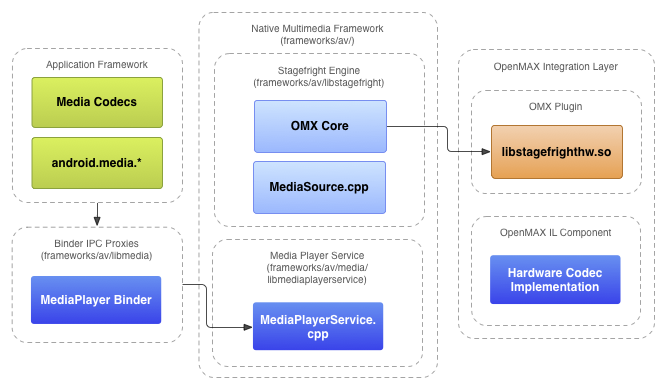
\includegraphics[width=350px]{video_decoding/native.png}
Apps can utilize the Stagefright framework by using the classes inside the android.media APIs\footnote{http://developer.android.com/reference/android/media/package-summary.html}. These classes communicate with the Stagefright framework by making use of the Binder\footnote{http://developer.android.com/reference/android/os/Binder.html} class which facilitates inter-process communication. As mentioned, Stagefright comes with built-in software codecs, and can be extended with hardware-based OpenMAX(OMX) codecs, called components. An additional shared library, an OpenMax plugin, links these codecs to Stagefright.
\subsection{Documentation}
Extensive documentation, including API guides and references, is available through the official android developer portal.\footnote{http://developer.android.com/develop/index.html}
\subsection{Updates}
The Stagefright multimedia framework is updated with every new android version, and up-to-date hardware video codecs are supplied with it by the mobile device vendors.
\subsection{Performance}
Stagefright offers excellent performance, especially given its hardware acceleration support. It is a production quality framework that has not shown any bugs so far.


